% Created 2020-11-10 Tue 10:18
% Intended LaTeX compiler: pdflatex
\documentclass[11pt]{article}
\usepackage[utf8]{inputenc}
\usepackage[T1]{fontenc}
\usepackage{graphicx}
\usepackage{grffile}
\usepackage{longtable}
\usepackage{wrapfig}
\usepackage{rotating}
\usepackage[normalem]{ulem}
\usepackage{amsmath}
\usepackage{textcomp}
\usepackage{amssymb}
\usepackage{capt-of}
\usepackage{hyperref}
\author{Jeroen de Haas}
\date{\today}
\title{Een libkmint tutorial}
\hypersetup{
 pdfauthor={Jeroen de Haas},
 pdftitle={Een libkmint tutorial},
 pdfkeywords={},
 pdfsubject={},
 pdfcreator={Emacs 27.1 (Org mode 9.3.7)}, 
 pdflang={English}}
\begin{document}

\maketitle
\tableofcontents


\section{Introductie}
\label{sec:org677476d}
\texttt{libkmint} is een C++-bilbiotheek waarmee je de opdrachten voor het vak
kunstmatige intelligentie kan maken. Het staat je vrij om een andere
bibliotheek te gebruiken of zelf iets te schrijven zolang de bibliotheek van
jouw keuze de technieken die in dit vak worden behandeld niet al
implementeert.

\section{Structuur van het project}
\label{sec:org55d0fab}
Het project op Blackboard is onderverdeeld in een bibliotheek \texttt{libkmint} en
een applicatie \texttt{kmintapp}. Daarnaast bevat de map \texttt{dependencies} de SDL2 en
SDL2\textsubscript{image} bibliotheek voor Windows. Linux- en macOS-gebruikers moeten deze
bibliotheken via een \emph{package manager} installeren.

Je plaatst jouw eigen bronbestanden in de map \texttt{kmintapp/src}. De code onder
\texttt{libkmint} laat je best ongemoeid. Mochten jij of een van je collega's
namelijk een fout ontdekken, dan krijgen jullie van ons een nieuwe versie
van \texttt{libkmint}. 

Als je een cpp-bestand toevoegt aan \texttt{kmintapp/src} dan dien je ook
\texttt{kmintapp/CMakeLists.txt} aan te passen. In dat bestand vind je nu
onderstaande code:
\begin{verbatim}
add_executable(kmintapp
  src/main.cpp
  src/hare.cpp
  src/cow.cpp)
\end{verbatim}
Voeg je het bestand \texttt{astar.cpp} toe, moet deze als volgt aan het project
worden gekoppeld:
\begin{verbatim}
add_executable(kmintapp
  src/main.cpp
  src/astar.cpp # NIEUWE REGEL!
  src/hare.cpp
  src/cow.cpp)
\end{verbatim}

\textbf{Let op:} Headers moeten \emph{niet} aan het project worden gekoppeld. Deze
worden indirect meegenomen via \texttt{include}-directives.

\subsection{CLion}
\label{sec:org7d75c18}
Het project kan onder Linux en macOS met CLion worden geopend en
gecompileerd. De combinatie van CLion en Windows is niet getest.

\subsection{Visual Studio}
\label{sec:orgaaac59a}
Onder Windows wordt Visual Studio 2017 ondersteund. Om het
project in Visual Studio 2017 te openen kies je "File -> Open -> CMake" en
selecteer je het \texttt{CMakeLists.txt} bestand in de hoofdmap. \textbf{Let op:} Open niet
de gelijknamige bestanden in de mappen \texttt{kmintapp} of \texttt{libkmint}. 

Kies na het openen \texttt{kmintapp.exe} als "Startup Item" en druk op de knop met
het groene afspeelsymbool. Als het goed is verschijnt een zwart venster.




\section{Terminologie}
\label{sec:org34a10d8}
\texttt{libkmint} gebruikt de volgende begrippen:
\begin{description}
\item[{stage}] Een stage (\emph{podium}) is de spelwereld waarop zich alle agenten
bevinden. In de regel geldt dat alles wat beweegt, interageert
met de wereld of getekend moet worden op het podium geplaatst
moet worden.
\item[{actor}] Een actor (\emph{acteur}) staat op het podium. Je agenten (de koe en
de haas) zijn actors. Daarnaast zijn zaken als de achtergrond van
de speelwereld en de graaf ook actors. Actors hoeven dus niet
dynamisch van aard te zijn.
\item[{drawable}] Elke actor moet gekoppeld zijn aan een \texttt{drawable}. \texttt{drawable}
is een basisklasse voor objecten die getekend worden op het
scherm. Afgeleide klassen moeten de functie \texttt{draw}
implementeren waarin getekend wordt.
\item[{graph}] een graph representeert een graaf.
\item[{map}] een map, oftewel kaart, is een combinatie van een graaf en een
afbeelding die dient als achtergrond.
\end{description}



\section{Hello, world}
\label{sec:org5ae16de}
Hieronder staat een simpel "hello world"-programma dat een venster opent en
wacht tot de gebruiker op de \texttt{q} drukt:

\begin{verbatim}
 1  #include "kmint/graphics.hpp"      // kleuren en afbeeldingen
 2  #include "kmint/main.hpp"          // voor de main loop
 3  #include "kmint/math/vector2d.hpp" // voor window en app
 4  #include "kmint/play.hpp"          // voor stage
 5  #include "kmint/ui.hpp"            // voor window en app
 6  
 7  using namespace kmint; // alles van libkmint bevindt zich in deze namespace
 8  
 9  int main() {
10    // een app object is nodig om
11    ui::app app{};
12  
13    //  maak een venster aan
14    ui::window window{app.create_window({1024, 768}, "hello")};
15  
16    // maak een podium aan
17    play::stage s{};
18  
19    // Maak een event_source aan (hieruit kun je alle events halen, zoals
20    // toetsaanslagen)
21    ui::events::event_source event_source{};
22  
23    // main_loop stuurt alle actors aan.
24    main_loop(s, window, [&](delta_time dt, loop_controls &ctl) {
25      // gebruik dt om te kijken hoeveel tijd versterken is
26      // sinds de vorige keer dat deze lambda werd aangeroepen
27      // loop controls is een object met eigenschappen die je kunt gebruiken om de
28      // main-loop aan te sturen.
29  
30      for (ui::events::event &e : event_source) {
31        // event heeft een methjode handle_quit die controleert
32        // of de gebruiker de applicatie wilt sluiten, en zo ja
33        // de meegegeven functie (of lambda) aanroept om met het
34        // bijbehorende quit_event
35        //
36        e.handle_quit([&ctl](ui::events::quit_event qe) {
37          ctl.quit = true;
38        });
39        e.handle_key_up([&ctl, &my_actor](ui::events::key_event k) {
40          // jouw code hier
41        });
42      }
43    });
44  }
\end{verbatim}

\section{Een actor toevoegen}
\label{sec:orge966c3a}
In deze paragraaf voegen we een actor toe aan de spelwereld. Een actor moet
de van de klasse \texttt{kmint::play::actor} overerven. In dit voorbeeld erven we
over van \texttt{free\_roaming\_actor}, een basisklasse voor actors die op een
willekeurige positie kunnen staan.

Om een actor te tekenen, moet je daarnaast een klasse maken die is afgeleid
van \texttt{kmint::ui::drawable}. Deze abstracte klasse bevat een methode \texttt{draw}
die elk frame wordt aangeroepen. Via de meegegeven \texttt{frame} referentie kun je
tekenen. Onderstaande code bevat de code voor een simpele \texttt{drawable} en een
eerste \texttt{actor}.


\begin{verbatim}
class rectangle_drawable : public ui::drawable {
public:
  rectangle_drawable(play::actor const &actor) : drawable{}, actor_{&actor} {}
  void draw(ui::frame &f) const override;

private:
  play::actor const *actor_;
};

void rectangle_drawable::draw(ui::frame &f) const {
  f.draw_rectangle(actor_->location(), {10.0, 10.0}, graphics::colors::white);
}

class hello_actor : public play::free_roaming_actor {
public:
  hello_actor(math::vector2d location)
      : free_roaming_actor{location}, drawable_{*this} {}

  const ui::drawable &drawable() const override { return drawable_; }

private:
  rectangle_drawable drawable_;
};
\end{verbatim}

Om deze actor op je \texttt{stage} te plaatsen, gebruik je de functie
\texttt{stage::build\_actor}. Deze functie bouwt een actor en geeft een referentie
naar de gebouwde \texttt{actor} terug. Jouw code zal dus \emph{nooit} de eigenaar zijn
van welke \texttt{actor} dan ook. Het eigendom van deze objecten ligt bij
\texttt{stage}. Verander onderstaand stukje van je \texttt{main} functie:
\begin{verbatim}
// maak een podium aan
play::stage s{};
\end{verbatim}
in 
\begin{verbatim}
// maak een podium aan
play::stage s{};

math::vector2d center{512.0, 384.0};
auto &my_actor = s.build_actor<hello_actor>(center);
\end{verbatim}


\section{Interactie}
\label{sec:org2cb7042}
Voeg onderstaande functie toe aan \texttt{hello\_actor}:
\begin{verbatim}
void move(math::vector2d delta) { location(location() + delta); }
\end{verbatim}

Pas de for-lus aan in \texttt{main\_loop}:
\begin{verbatim}
for (ui::events::event &e : event_source) {
  // event heeft een methode handle_quit die controleert
  // of de gebruiker de applicatie wilt sluiten, en zo ja
  // de meegegeven functie (of lambda) aanroept om met het
  // bijbehorende quit_event
  //
  e.handle_quit([&ctl](ui::events::quit_event qe) { ctl.quit = true; });
  e.handle_key_up([&my_actor](ui::events::key_event k) {
    switch (k.key) {
    case ui::events::key::up:
      my_actor.move({0, -5.0f});
      break;
    case ui::events::key::down:
      my_actor.move({0, 5.0f});
      break;
    case ui::events::key::left:
      my_actor.move({-5.0f, 0});
      break;
    case ui::events::key::right:
      my_actor.move({5.0f, 0});
      break;
    default:
      break;
    }
  });
}
\end{verbatim}

Als het goed is, kun je het vierkantje nu verplaatsen met de pijltjes toetsen!

\section{Een kaart toevoegen}
\label{sec:org88e17dd}

Een kaart is een combinatie van een graaf met een achtergrondafbeelding. Een kaart
is een tweedimensionaal grid van vakjes. Een deel van deze vakjes zijn
verbonden met hun linker-, rechter-, boven- en/of onderbuur. Zo vormen deze
vakjes samen een graaf.

Een kaart wordt ingelezen uit een string. Hieronder zie je een voorbeeld,
verderop wordt per regel uitgelegd waar deze voor staat.
\begin{verbatim}
 1  40 6 32
 2  resources/map3.png
 3  G 1 1
 4  C 1 2
 5  W 0 0
 6  B 1 8
 7  
 8  GGGGGGGGGGGGGGGGGGGGGGGGGGGGGGGGGGGGGGGG
 9  GGGGGGGGGGGGGGGGGGGGGGGGGGGGGGGGGGGGGGGG
10  GGGGGGGGGGGGGGGGGGGGGGGGGGCCCCCGGGGGGGGG
11  GGGGGGGGGGGGGGGGGGGGGGGGGGCCCCCGGGGGGGGG
12  GGGGGGGGGGGGGGGGGGGGGGGGGGCCCCCGGGGGGGGG
13  WWWWWWWWWBWWWWWWWWWWWWGGGGGGGGGGGGGGGGGG
\end{verbatim}

\begin{description}
\item[{1}] De afmetingen van de kaart. Deze kaart is 40 vakjes breed, 6 vakjes
hoog en elk vakje is 32 bij 32 pixels groot
\item[{2}] Het pad naar de achtergrondafbeelding
\item[{3 t/m 6}] Een beschrijving van de vakjes. Elk vakje heeft een symbool
('G', 'C', 'W' of 'B'). Dit symbool wordt gevolgd door een 0 of
een 1 die aangeeft of het vakje begaanbaar is. Een 0 betekent
niet begaanbaar, een 1 betekent begaanbaar. Het laatste getal
geeft hoe moeilijk het is om over dit vakje te bewegen. Het
kost twee maal zoveel tijd om een vakje met een
moeilijkheidsgraad van 2 te verlaten.
\item[{7}] Een witregel die de informatie over de kaart scheidt van de echte kaart
\item[{8 t/m 13}] Een beschrijving van de kaart. Elke regel correspondeert met
een rij op de kaart, elk symbool met een vakje.
\end{description}

\subsection{Inlezen}
\label{sec:org7a56737}
Om een kaart uit te lezen is het noodzakelijk volgende header te in te voegen:
\begin{verbatim}
#include "kmint/map/map.hpp"
\end{verbatim}

De definitie van een kaart kun je direct in je programma
plaatsen. Onderstaande code laat zien hoe je dit met behulp van een \emph{raw
string literal\footnote{Zie \href{https://en.cppreference.com/w/cpp/language/string\_literal}{dit voorbeeld op cppreference.com}.}} kunt doen:
\begin{verbatim}
static const char *map_description = R"graph(32 24 32
resources/firstmap.png
G 1 1
C 1 1
H 1 1
W 0 0
B 1 8

WWWWWWWWWWWWWWWWWWWWWWWWWWWWWWWW
WWWWWWWWWWWWWWWWWWWWWWWWWWWWWWWW
WWWWWWWWWWWWWWWWWWWWWWWWWWWWWWWW
WWWHGGGGGGGGGGGGGGGGGGGGGGGGHWWW
WWWGGGGGGGGGGGGGGGGGGGGGGGGGGWWW
WWWGGGGGGGGGGGGGBGGGGGGGGGGGGWWW
WWWGGGGGGWWWWWWWBWWWWWWGGGGGGWWW
WWWGGGGGGWWWWWWWBWWWWWWGGGGGGWWW
WWWGGGGGGWWWWWWWBWWWWWWGGGGGGWWW
WWWGGGGGGWWWWWGGBGWWWWWGGGGGGWWW
WWWGGGGGGWWWWWGGGGWWWWWGGGGGGWWW
WWWGGGGGGWWWWWGGGGWWWWWGGGGGGWWW
WWWGGGGGBBBBBBBGCGGGGGGGGGGGGWWW
WWWGGGGGGWWWWWGGGGWWWWWGGGGGGWWW
WWWGGGGGGWWWWWGGBGWWWWWGGGGGGWWW
WWWGGGGGGWWWWWWWBWWWWWWGGGGGGWWW
WWWGGGGGGWWWWWWWBWWWWWWGGGGGGWWW
WWWGGGGGGWWWWWWWBWWWWWWGGGGGGWWW
WWWGGGGGGGGGGGGGBGGGGGGGGGGGGWWW
WWWGGGGGGGGGGGGGGGGGGGGGGGGGGWWW
WWWHGGGGGGGGGGGGGGGGGGGGGGGGHWWW
WWWWWWWWWWWWWWWWWWWWWWWWWWWWWWWW
WWWWWWWWWWWWWWWWWWWWWWWWWWWWWWWW
WWWWWWWWWWWWWWWWWWWWWWWWWWWWWWWW
)graph";
\end{verbatim}

Met volgende code lees je de kaart vervolgens uit:
\begin{verbatim}
map::map m{map::read_map(map_description)};
\end{verbatim}

De afbeelding en de graaf moeten elk onafhankelijk worden
getekend. Hiervoor gebruik je twee verschillende soorten actors. Een
\texttt{map\_actor} tekent de graaf die hoort bij de kaart, en een \texttt{background}
tekent de achtergrond. Zorg ervoor dat je eerst de background aan je stage
toevoegt, gevolgd door de graaf. Daarna kun je andere actors toevoegen:
\begin{verbatim}
s.build_actor<play::background>(
  math::size(1024, 768),
  graphics::image{m.background_image()});
s.build_actor<play::map_actor>(
  math::vector2d{0.0f, 0.0f},
  m.graph());
\end{verbatim}

Als het goed is, zie je nu volgend programma:

\begin{center}
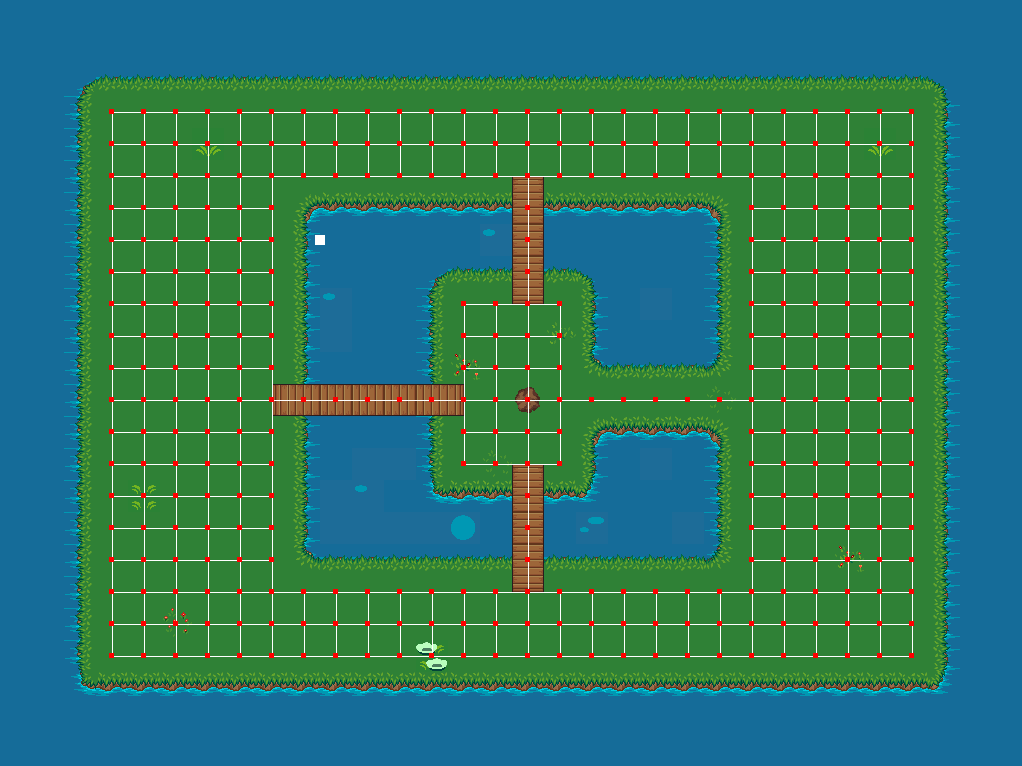
\includegraphics[width=.9\linewidth]{./resources/screenshot.png}
\end{center}

\subsection{De structuur van een kaart}
\label{sec:orgbf83952}
Een \texttt{map} bestaat uit twee delen, een graaf van het type \texttt{map\_graph} en het
pad naar een achtergrondafbeelding. De graaf haal je op via de functie
\texttt{map::graph()}. Deze graaf kun je zien als een array van knopen van het
type \texttt{map\_node}. Het aantal knopen in een kaart kun je opvragen met de
functie \texttt{map\_graph::num\_nodes()}. De nodes kun je ophalen met de subscript
operator, bijvoorbeeld zo:
\begin{verbatim}
// laad een kaart
map::map m{map::read_map(map_description)};
auto &graph = m.graph();
for (std::size_t i = 0; i < graph.num_nodes(); ++i) {
  std::cout << "Knoop op: " << graph[i].location().x() << ", "
            << graph[i].location().y() << "\n";
}
\end{verbatim}

Een knoop kun je op zijn beurt weer zien als een array van kanten van het
type \texttt{map\_edge}. Het aantal kanten aan een knoop vraag je op met
\texttt{map\_node::num\_edges} en met de subscript operator kun je een van de kanten opvragen:
\begin{verbatim}
auto &node = graph[0];
for (std::size_t i = 0; i < node.num_edges(); ++i) {
  auto &from = node[i].from();
  auto &to = node[i].to();
  std::cout << "Kant van: " << from.location().x() << ", "
            << from.location().y() << " naar " << to.location().x() << ", "
            << to.location().y() << "\n";
}
\end{verbatim}

Elke kant heeft een gewicht. Dit geeft aan hoe lastig het is voor een actor
om zich via die kant te verplaatsen. De kanten horende bij de brug hebben
een gewicht van acht. Je kunt het gewicht ophalen met de functie \texttt{weight}:
\begin{verbatim}
auto &node = graph[0];
auto &edge = node[0];
float weight = edge.weight();
\end{verbatim}

\textbf{Voor gevorderden:} Wil je deze klassen gebruiken in combinatie met
STL-algoritmen dan kan dat. \texttt{map\_graph} en \texttt{map\_node} bieden member
functions \texttt{begin} en \texttt{end} die de juiste iterators teruggeven.


\section{Een actor op de graaf}
\label{sec:orgab4831a}
Een volgende stap is om een actor te laten bewegen over de graaf. In het
midden van de kaart zie je een modderhoop. In de tekstuele beschrijving van
de kaart is dit punt met de letter \texttt{C} aangegeven. Dit is het vertrekpunt van de
koe. Zij zal het eiland vanuit dit punt over het eiland gaan dwalen.

Eerst schrijven we een functie die de de kaart afzoekt naar het beginpunt
van de koe:
\begin{verbatim}
const map::map_node &find_cow_node(const map::map_graph &graph) {
  for (std::size_t i = 0; i < graph.num_nodes(); ++i) {
    if (graph[i].node_info().kind == 'C') {
      return graph[i];
    }
  }
  throw "could not find starting point";
}
\end{verbatim}

In onze \texttt{main} functie roepen we deze functie aan
\begin{verbatim}
auto &cow_node = find_cow_node(m.graph());
\end{verbatim}


Actors die zich over de kaart bewegen worden afgeleid van de klasse
\texttt{map\_actor}. We maken nu een klasse koe die elke seconde een stap op de
kaart zet. Hiervoor maken we een header \texttt{cow.hpp} en een bronbestand,
\texttt{cow.cpp} aan. In \texttt{cow.hpp} plaats je volgende code:
\begin{verbatim}
#ifndef KMINTAPP_COW_HPP
#define KMINTAPP_COW_HPP

#include "kmint/map/map.hpp"
#include "kmint/play.hpp"
#include "kmint/primitives.hpp"

class cow : public kmint::play::map_bound_actor {
public:
  cow(kmint::map::map_graph const &g, kmint::map::map_node const &initial_node);
  // wordt elke game tick aangeroepen
  void act(kmint::delta_time dt) override;
  kmint::ui::drawable const &drawable() const override { return drawable_; }
  // als incorporeal false is, doet de actor mee aan collision detection
  bool incorporeal() const override { return false; }
  // geeft de radius van deze actor mee. Belangrijk voor collision detection
  kmint::scalar radius() const override { return 16.0; }

private:
  // hoeveel tijd is verstreken sinds de laatste beweging
  kmint::delta_time t_passed_{};
  // weet hoe de koe getekend moet worden
  kmint::play::image_drawable drawable_;
  // edge_type const *next_edge_{nullptr};
  // edge_type const *pick_next_edge();
};

#endif /* KMINTAPP_COW_HPP */
\end{verbatim}

\texttt{cow.cpp} ziet er als volgt uit:
\begin{verbatim}
#include "cow.hpp"
#include "kmint/random.hpp"
using namespace kmint;

static const char *cow_image = "resources/cow.png";
cow::cow(map::map_graph const &g, map::map_node const &initial_node)
    : play::map_bound_actor{g, initial_node}, drawable_{*this,
                                                        kmint::graphics::image{
                                                            cow_image, 0.1}} {}

void cow::act(delta_time dt) {
  t_passed_ += dt;
  if (to_seconds(t_passed_) >= 1) {
    // pick random edge
    int next_index = random_int(0, node().num_edges());
    this->node(node()[next_index].to());
    t_passed_ = from_seconds(0);
  }
}
\end{verbatim}

Laad \texttt{cow.hpp} vervolgens in \texttt{main.cpp}:
\begin{verbatim}
#include "cow.hpp"
\end{verbatim}

En plaats de koe op het podium:
\begin{verbatim}
s.build_actor<cow>(m.graph(), cow_node);
\end{verbatim}


\section{Collision detection}
\label{sec:orgec05289}
Naast de koe bevindt zich ook een haas op de kaart. De koe moet deze haas
vangen. De haas bevindt zich op een van de vier uithoeken van de kaart, deze
zijn te herkennen aan de \texttt{H} in de tekstuele representatie.

De haas is een \texttt{map\_bound\_actor}. De header file voor de haas wordt \texttt{hare.hpp}:
\begin{verbatim}
#ifndef KMINTAPP_HARE_HPP
#define KMINTAPP_HARE_HPP

#include "kmint/map/map.hpp"
#include "kmint/play.hpp"
#include "kmint/primitives.hpp"
#include "kmint/random.hpp"

class cow;

class hare : public kmint::play::map_bound_actor {
public:
  hare(kmint::map::map_graph const &g);
  void act(kmint::delta_time dt) override;
  kmint::ui::drawable const &drawable() const override { return drawable_; }
  void set_cow(cow const &c) { cow_ = &c; }
  bool incorporeal() const override { return false; }
  kmint::scalar radius() const override { return 16.0; }

private:
  kmint::play::image_drawable drawable_;
  cow const *cow_;
};

#endif /* KMINTAPP_HARE_HPP */
\end{verbatim}

De haas blijft net zolang staan tot de koe haar vangt. Op dat moment wordt
ze verplaatst naar een andere geschikte locatie. De haas wordt als volgt
geïmplementeerd:
\begin{verbatim}
#include "hare.hpp"
#include "cow.hpp"
#include "kmint/random.hpp"

using namespace kmint;

static const char *hare_image = "resources/hare.png";

map::map_node const &random_hare_node(map::map_graph const &graph) {
  int r = kmint::random_int(0, 3);
  for (std::size_t i = 0; i < graph.num_nodes(); ++i) {
    if (graph[i].node_info().kind == 'H') {
      if (r == 0)
        return graph[i];
      else
        --r;
    }
  }
  throw "could not find node for hare";
}

hare::hare(map::map_graph const &g)
    : play::map_bound_actor{g, random_hare_node(g)},
      drawable_{*this, kmint::graphics::image{hare_image}} {}

void hare::act(kmint::delta_time dt) {
  for (std::size_t i = 0; i < num_colliding_actors(); ++i) {
    auto &a = colliding_actor(i);
    if (&a == cow_) {
      node(random_hare_node(graph()));
    }
  }
}
\end{verbatim}

Pas tenslotte de code in \texttt{main.cpp} aan opdat de haas weet wie de koe is. De
code die de koe en de haas op het podium plaatst hoort er als volgt uit te
zien:
\begin{verbatim}
auto &cow_node = find_cow_node(m.graph());
auto &my_cow = s.build_actor<cow>(m.graph(), cow_node);
auto &my_hare = s.build_actor<hare>(m.graph());
my_hare.set_cow(my_cow);
\end{verbatim}

\section{The end}
\label{sec:org4252455}
Je hebt nu een werkend basisprogramma waarmee je aan de opdrachten voor week
1 kunt gaan werken. Succes!
\end{document}
